% #########################################################################################
% #########################################################################################
% #########################################################################################
\section{Exercise design}

% -----------------------------------------------------------------------------------------
\subsection{Description of the tested functionality}

In the present work, we focus on the impact of using a \gls{FLM} or a \gls{FF} approach. 

A \gls{FLM} approach consists to adapt the fresh fuel composition according to
the reactor requirements and the available isotopes. A \gls{FLM} means there is a
process that connects the fresh fuel composition to the available materials,
whatever the complexity of the model. For instance, the fissile fraction is
calculated from the fissile stock quality in order to reach the required burn-up
of the reactor. A \gls{FLM} could be based on neural network, Plutonium
equivalence model, analytic functions, built-in depletion, etc. A \gls{FLM} is
usually built from physics constraints and reactor physics calculations. 

A \gls{FF} approach consists in using the same constant fissile
fraction at each fresh fuel loading whatever the isotopic vector of the
available fissile material is. Using a PWR MOX which is always loaded with a
fresh fuel that contains 7\% of plutonium regardless the $^{239}$Pu content is a
\gls{FF} approach. 

The present work aims to quantify the impact of using \gls{FLM} versus \gls{FF}
approach considering this last one as the reference. In a fuel cycle code, the
\gls{FF} approach is the easiest method to handle fresh fuel loading in a reactor. The
user simply define explicitly the fuel composition that is used in all the
simulation. Developing \gls{FLM} may be an important development process that
may require time and effort. Testing the impact of using \gls{FLM} rather than
\gls{FF} approach aims to show applications that need \gls{FLM} and study that can be
solved with \gls{FF} approach.

\subsection{Output of interest}

Fuel fabrication models can impacts fuel cycle simulation in different ways.
This exercise aims to understand some of their impacts on an overall fuel cycle
calculation. Change in the plutonium content in a newly built MOX fuel will
impacts the fuel cycle in 3 majors ways:

\begin{itemize}
    \item the global amount of plutonium in the simulation, variation in the
        plutonium content in the MOX fuel, might lead in a increase of the
        amount of plutonium burnt in the PWR reactor, or a change in the
        breeding/burning ratio in a SFR reactor, impacting the overall amount of
        plutonium in the simulation.
    \item the location of the plutonium, indeed the amount of plutonium in the
        MOX fuel will shift the localization of the plutonium form the front-end
        the back-end of the cycle, which could change its availability for
        other use (deployment of new reactor, fabrication of other fuels\ldots),
    \item the variation of the global amount of plutonium relative to the amount
        loaded in the fuel, the breeding/burning ratio of the plutonium will
        change the amount of plutonium in reactor.
\end{itemize}

This might not be exhaustive list of fuel fabrication models impact on a fuel
cycle, but this work will only focus on them and will not consider potential
consequence on the fuel composition change after depletion due to
over/under-estimate the amount of plutonium in the MOX fuel.

In order to investigate those impacts across multiple fuel cycle simulation tool
and associated models, the following experience has been designed.

% -----------------------------------------------------------------------------------------
\subsection{Exercise specifications}

The exercise is divided in two independent parts related to the reactor involved. \gls{PWR} and \gls{SFR} will be considered in this work.

The schematic representation of the fuel cycle is shown on Figure~\ref{fig:FuelCycle}. The fuel cycle includes a fissile stock that contains enough plutonium to operate one reactor cycle and a fertile stock filled of depleted uranium. A fresh fuel fabrication plant that uses the heavy elements of the stocks build the fresh fuel of the reactor (PWR or SFR) according the its technical requirements. The reactor spent fuel is sent to a dedicated stock.

\begin{figure}[h]
    \begin{center}
        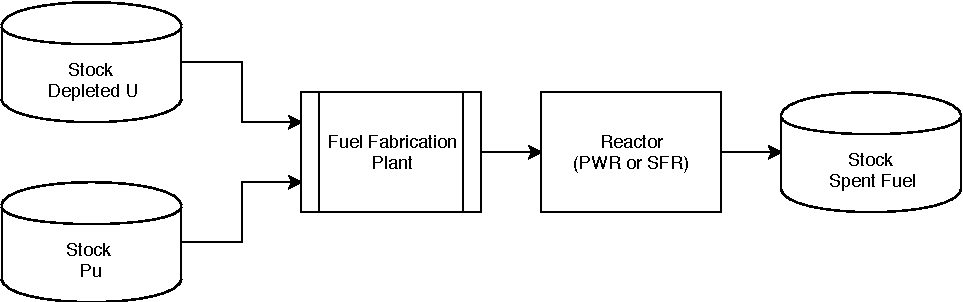
\includegraphics[width = 0.99\textwidth]{FIG/FuelCycleDiagram.pdf}
        \caption{Representation of the simulated fuel cycle facilities.}
        \label{fig:FuelCycle}
    \end{center}
\end{figure}

The time frame of the simulation corresponds to the reactor cycle. From the relation between the fuel cycle time $\Delta t$, the reactor thermal power $P_{th}$, the heavy nuclide mass $M$ and the reactor burn-up $BU$, we have : 

\begin{equation}
    \Delta t = \frac{BU \; M}{P_{th}}
\end{equation}

At t = 0, the fabrication plant builds the fresh fuel according to reactor requirements. To avoid plutonium isotopes decay, the fabrication time is zero and the reactor is thus loaded instantaneously. A complete fuel cycle is run and the spent fuel is sent to stock when the required BU is reached.

Concerning the plutonium vector used to build the MOX fuel, a large range has been imposed for plutonium isotopes. Indeed, the impact of a \gls{FLM} in relation to \gls{FF} approach on a fuel cycle calculation will increase with the plutonium fraction deviation from a reference case. To take an example, let consider a small fissile content plutonium. A \gls{FF} approach would for instance load the fuel at 6\% of plutonium in the fresh fuel since a \gls{FLM} approach would give 12\%. On the other hand, if the plutonium vector used to build the fuel is very close from the reference plutonium used to design the \gls{FF} approach, \gls{FF} and \gls{FLM} would produce similar results. Perfectly well tuned scenario for which plutonium stocks are well known and approximately constant with time can be properly solved with a \gls{FF} approach. 

A wide range of scenario applications is considered here. For instance, the plutonium vector produced from a small burn-up discharge CANDU is characterized by a high fissile fraction~\cite{Guillemin_2010}. The multi-recycling of the plutonium into PWR may produce a high even isotopes fraction in the plutonium vector~\cite{Courtin_2016}. Very specific plutonium isotopic fraction can be seen from scenarios involving SFR reactors. Also, industrial parameters, such has spent fuel cooling time, may have a strong impact on $^{241}$Pu fraction. For those reasons, the plutonium isotopic range has been chosen very large to be representative of a wide range of applications although being realistic enough. The Table~\ref{Tab:PuVector} present minimum and maximum isotopic fraction of plutonium isotopes used in the framework of this work.

\begin{table}[h]
\centering
\begin{tabular}{ |l|l|l| }
  \hline
  Isotope & Min. Mass Fr. (wgt. \%) & Max. Mass Fr. (wgt. \%) \\
  \hline
  Pu-238/TRU & 0  & 10 \\
  \hline
  Pu-239/TRU & 25 & 90 \\
  \hline
  Pu-240/TRU & 10 & 40 \\
  \hline
  Pu-241/TRU & 0  & 25 \\
  \hline
  Pu-242/TRU & 0  & 30 \\
  \hline
  Am-241/TRU & 0  & 10 \\
  \hline
\end{tabular}
\label{Tab:PuVector}
\caption{Minimum and maximum mass fraction in weight \% for plutonium vector at reactor beginning of cycle used in the framework of this work}
\end{table}

% -----------------------------------------------------------------------------------------
\subsection{Problem-solving methodology}

In order to investigate the influence of using a \gls{FLM} rather than a
\gls{FF} approach on fuel cycle simulations, the following experiment have been
designed. Following the FIT project spirit, no code to code comparison will be
done. For each simulator used to solve this problem, fuel models will be
compared within the same simulator, allowing to evaluate difference between two
almost identical simulation: same simulator, reactor description, depletion
algorithm, \ldots the only difference being the method used to build the fresh fuel.

The experiment consists in running a small fuel cycle calculation according to
specifications defined above. We use a method that we call "Wide Parametric
Sweeping" method. The principle of this method is to fill from a random 
sampling method the plutonium isotopic space defined in the Table~\ref{
Tab:PuVector}. The global set of plutonium isotopic vectors that will be run 
is called the design of experiment. Each plutonium isotopic vector will be run 
twice. One using a \gls{FLM} approach for which the plutonium fraction at 
reactor \gls{BOC} directly depends on the plutonium isotopic composition. The 
second run uses \gls{FF} approach for which the plutonium fraction at \gls{BOC}
is always the same. 

Each code produces for each reactor, \gls{PWR} and \gls{SFR}, two sets of output data representing \gls{FLM} and \gls{FF} runs. For each case, the output of interest are the mass of plutonium at \gls{BOC} $M_{Pu}^{BOC}$ and \gls{EOC} $M_{Pu}^{BOC}$ and the plutonium fraction $\lambda_{\mathrm{Pu}}^{BOC}$ at \gls{BOC}. Future works will be dedicated to extend the range of output, up to plutonium isotopic composition or minor actinides production. 

In order to measure the influence of the use of \gls{FF} versus \gls{FLM} on the global amount of plutonium in the simulation, the location
of the plutonium and the speed of variation of the plutonium inventory, three
estimators have been defined.

\subsection{Estimators}

From output data of interest, estimators are built to compare simulations run from \gls{FF} and \gls{FLM}. Inside a fuel cycle, two effects are dissociated. The first effect concerns global outputs which is a data estimated on the entire fuel cycle. This could be the total inventory of plutonium or minor actinides for for instance. The second effect concerns local outputs and is associated to the inventory in a specific facility or disposal unit. This could be the plutonium mass in a strategic stock. A measured global effect necessarily induces a local effect. Indeed, if the total plutonium mass at a specific time calculated from \gls{FLM} approach is higher than the \gls{FF} approach, that means that one or more facilities are affected. On the contrary, a local effect does not necessarily mean there is a global effect. A deviation in plutonium mass in a specific stock can be compensated in another facility.

\subsubsection{Estimator 1}
The first estimator aims to measure the difference on the plutonium enrichment in the MOX
fuel between the \gls{FLM} and \gls{FF}. This estimator directly impacts the amount of
plutonium present in the back-end part of the fuel cycle and is then a local estimator. The estimator 1 has been defined as:

\begin{equation}
    \delta{\lambda}(i) =
        \frac{\left(\lambda_{\mathrm{Pu}}^{BOC}(i)\right)_{FML}
              - \left(\lambda_{\mathrm{Pu}}^{BOC}(i)\right)_{FF}}
              {\left(\lambda_{\mathrm{Pu}}^{BOC}(i)\right)_{FF}},
\end{equation}

where $\lambda_i$ represents the fraction of plutonium at \gls{BOC} or at
\gls{EOC} for the plutonium composition $i$ for the \gls{FLM} or the \gls{FF}. The higher the estimator 1 is, the higher the plutonium fraction at \gls{BOC} is for the \gls{FLM} compared to \gls{FF}. This estimator is used in the case of \gls{PWR} and \gls{SFR} analysis.

\subsubsection{Estimator 2}

The second estimator aims to estimate the relative speed of plutonium consumption in the reactor between the \gls{FLM} and the \gls{FF} approach. The estimator 2 is defined as:

\begin{equation}
    \delta{\frac{\Delta M}{M}}(i) =
        \frac{\left(\frac{\Delta M}{M}(i)\right)_{FML}
              - \left(\frac{\Delta M}{M}(i)\right)_{FF}}
             {\left(\frac{\Delta M}{M}(i)\right)_{FF}},
\end{equation}
where $\frac{\Delta M}{M}_{i}$ is defined as:
\begin{equation}
    \frac{\Delta M}{M}(i) = \frac{M_{Pu}^{BOC}(i) -
    M_{Pu}^{EOC}(i)}{M_{Pu}^{BOC}(i)}
\end{equation}

Estimator 2 represents a global effect since the plutonium consumption speed has an impact on total plutonium mass. This estimator is suitable for reactor simulations characterized by plutonium decrease and is used for PWR analysis.

\subsubsection{Estimator 2b}

The estimator 2 can tend toward infinity if reactor is iso-breeder. To avoid such a behavior, an estimator 2b has been defined as following : 

\begin{equation}
    \delta \frac{\Delta M}{M}(Pu_i) = \frac{\Delta M}{M}(Pu_i)_{FLM} - \frac{\Delta M}{M}(Pu_i)_{FF}
\end{equation}

Estimator 2b measures a global effect and will be used for \gls{SFR} results.

\subsubsection{Estimator 3}

The third estimator shows the absolute speed of plutonium consumption in the reactor between the \gls{FLM} and the \gls{FF} approach and is defined as following :

\begin{equation}
    \delta{\frac{\Delta M}{T}}(i) =
        \frac{\left(\frac{\Delta M}{T}(i)\right)_{FML}
              - \left(\frac{\Delta M}{T}(i)\right)_{FF}}
             {\left(\frac{\Delta M}{T}(i)\right)_{FF}},
\end{equation}
where $\frac{\Delta M}{T}_{i}$ is defined as:
\begin{equation}
    \frac{\Delta M}{T}(i) = \frac{M_{Pu}^{BOC}(i) -
    M_{Pu}^{EOC}(i)}{T}
\end{equation}

Estimator 3 characterizes a global effect and is used in the case of PWR simulations analysis.

% -----------------------------------------------------------------------------------------
\subsection{Output observables}


